\begin{figure}[htp]
	\begin{center}
	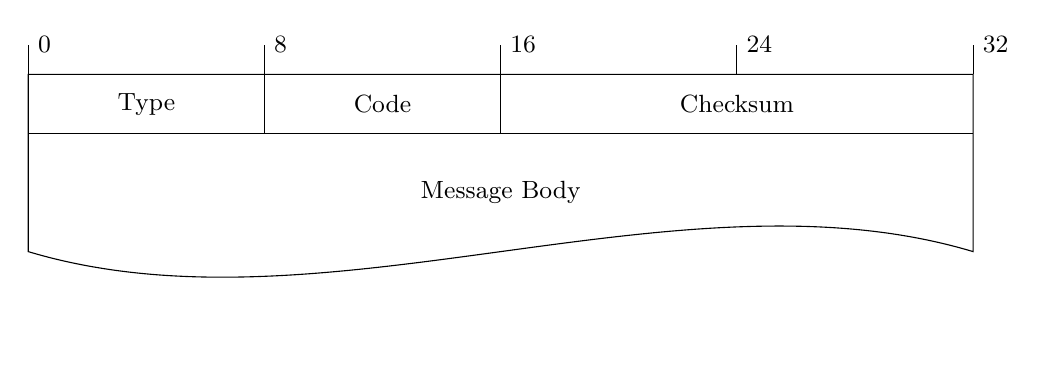
\begin{tikzpicture}[scale=0.75]
		\draw (0,0) .. controls (5, -1.5) and (11,1.5) .. (16,0) -- (16,3) -- (0,3) -- cycle;
		\draw (0,3) -- ++(0,0.5) node[right] {\small 0};
		\draw (4,3) -- ++(0,0.5) node[right] {\small 8};
		\draw (8,3) -- ++(0,0.5) node[right] {\small 16};
		\draw (12,3) -- ++(0,0.5) node[right] {\small 24};
		\draw (16,3) -- ++(0,0.5) node[right] {\small 32};

		\draw (4,2) -- ++(0,1);
		\node at (2,2.5) {\small Type};
		\draw (8,2) -- ++(0,1);
		\node at (6, 2.5) {\small Code};
		\node at (12, 2.5) {\small Checksum};
		\draw (0,2) -- ++(16,0);

		\node at (8,1) {\small Message Body};
	\end{tikzpicture}
	\end{center}
	\caption{Internet Control Message Protocol Format}
	\label{fig:icmp_format}
\end{figure}